\documentclass[11pt]{jreport}
\usepackage{wusepre_thesis}
\usepackage{indentfirst}
\usepackage{array}
\usepackage{amsmath}
\usepackage{newtxtext,newtxmath}
\usepackage{ascmac}
\usepackage{here}
\usepackage{mathtools}
\usepackage{slashbox}
\usepackage{multirow}
\usepackage{cancel}
\usepackage{framed}
\usepackage{graphicx}
\usepackage{url}	% \url{}コマンド用.URLを表示する際に便利
			% 他のパッケージ・スタイルを使う場合には適宜追加
			% 高専のころ使ってたもの何個か追加

%%%%%%%%%%%%%%%%%%%%%%%%%%%%%%%%%%%%%%%%%%%%%%%%%%%%%%%%%%%%%%%%%%%%%%%%

%%
%% 主に表紙を作成するための情報
%%

%%  タイトル(修論の場合は英語表記も指定)
\title{任意方向のカメラ移動を伴うモーションキャプチャ \\
        及び端末の自己位置推定の手法}
%\etitle{Test\\Test\\Test}

%%  著者名(修論の場合は英語表記も指定)
\author{高野 源太}
%\eauthor{Naoki Fukuyasu}

%% 卒業論文・修士論文(以下のどちらかを選択)
\prebachelar % プレ卒論(3年生用)
%\bachelar	% 卒業論文(4年生用)
%\master  	% 修士論文(M2用)

%%  学科・クラスタ
\department{システム工}
%\department{デザイン情報}
%\department{デザイン科学}

%%  学生番号
\studentid{60246336}

%%  卒業年度
\gyear{2021}		% 提出年が2021年なら,2020年度

%%  論文提出日
\date{2022年2月10日}	% 修士の場合は月(2021年2月)までとし,英語表記も指定
%\edate{February 2021}	% 修士の場合,こちら(英語表記)も有効化

%%%%%%%%%%%%%%%%%%%%%%%%%%%%%%%%%%%%%%%%%%%%%%%%%%%%%%%%%%%%%%%%%%%%%%%%

\begin{document}

\maketitle

%%
%%  概要
%%
\begin{abstract}


\end{abstract}

%%  目次
\tableofcontents

%%  図目次 (図目次をいれたければ以下のコメントをはずす)
%\listoffigures

%%  表目次 (表目次をいれたければ以下のコメントをはずす)
%\listoftables

\newpage
\pagenumbering{arabic}	% 以降のページ番号を算用数字に

%%%%%%%%%%%%%%%%%%%%%%%%%%%%%%%%%%%%%%%%%%%%%%%%%%%%%%%%%%%%%%%%%%%%%%%%

%%
%%  本文はここから
%%

\chapter{はじめに}
現在のスマホなどの単眼カメラが搭載された端末で行う光学式モーションキャプチャはカメラ位置を固定することが前提となっているものがほとんどであり、端末を動かしながらモーションキャプチャを行うといった利用方法は想定されていない。そのため、部屋内での端末の位置を推定し、端末の移動・カメラの向き等を考慮したモーションキャプチャの手法を確立することで、カメラ画角等にとらわれないモーションキャプチャを行うことができ、また、より簡易的にモーションキャプチャを利用することができるのではないかと考えた。

この研究では、部屋等の閉空間において一人の人間がカメラを持ちながらモーションキャプチャを行うといったような、単眼カメラの移動を考慮したモーションキャプチャの手法について検討する。通常単眼カメラによるモーションキャプチャにおいては、背景が固定となり、人間の動作から関節の動きを、もしくは人間の目の位置を判定し表情を画像認識等で抽出するという手法などがとられている。このため、カメラを動かすことを考えると人間と背景の境界の判定が精度面において必須になると考えられる。また、本手法では境界の判定を行ったあと人間の部分を除いた背景の情報及びスマホの回転角からスマホの自己位置推定を行う。

\chapter{関連研究}
本章では従来から研究されている単眼カメラを用いたモーションキャプチャの手法並びに障害物を考慮した自己位置推定(v-SLAM)の手法について述べる。

\section{単眼カメラを用いたモーションキャプチャの手法}\label{rep1}
本研究では、人の動きをデータとして取得するためにモーションキャプチャの手法のついて検討する。

単眼カメラを用いたリアルタイムでのモーションキャプチャの手法の一つとして、人体のシルエット画像並びに人体の肌色部分を抽出し、3次元モデルデータの骨格とマッチングさせるという手法がある[1]。この手法は、主に「顔位置の検出」、「肩位置の推定」、「人物領域・肌色領域の抽出」、「3次元位置の推定」の4ステップの工程によって成り立っており、フレーム毎に処理を行うと同時に、キャプチャが終了するまで4工程を繰り返し続けるものになっている。また、[1]では腕などの関節が多数あり、動きが多い部分の推定には、対象の動きを予測したサンプルを用いて対象の動きを逐次的に推定するパーティクルフィルタを適応するという手法がとられている。

さらに、動画像の場合(リアルタイムでは)、処理を行った直前の画像から整合性がとれるように骨格位置を修正する手法や近年ではAIに人の骨格及びその動きの情報を与え学習させ、様々な姿勢において検出ができるようにするといった手法[2]も取られており、後者においてはSDKやツールとして販売もされている。

\section{障害物を考慮した自己位置推定(v-SLAM)の手法}
Visual SLAMは、画像からカメラの位置姿勢と環境を同時に推定する手法である。このうち特徴点に基づく方法は、画像から検出した特徴点を追跡することによってカメラ位置の推定を行う。

このとき、移動する障害物(歩行者等)によって一部の特徴点が見えなくなる場合があると、照合ミスを起こし自己位置推定の破綻を起こす。このため、未知の障害物がある場合の位置推定を行う手法として\ref{rep1}節と同様にパーティクルフィルタを用いた手法が提案されている[3]。このパーティクルフィルタを用いた手法では、複数の特徴点を用いて推定される自己位置の候補(パーティクル)を複数仮定し、カメラの動きの情報などからそれぞれの候補の妥当性を調べて候補を絞るということを行う。また、自己位置推定を行う事前に、推定を行うエリアについて環境地図を作成し、壁などの既知の障害物の情報を取得するということを行っており、実際の測定でマッチングを行う際、取得した情報と環境地図の位置が合うように同次変換を行った後、ピクセルの差異を求めパーティクルの確からしさを判定する。

\chapter{使用機材・実装環境}
今回、研究をするにあたって利用を想定している環境及び機材を表\ref{jikkoukannkyou}に示す。

\begin{center}
\begin{table}[H]
\caption{使用する機材・実装環境}
\label{jikkoukannkyou}
\center
\begin{tabular}{|c||l|} \hline
言語 & Java(Kotlinも検討) \\ \hline 
開発OS & Windows  \\ \hline
統合開発環境(IDE) & AndroidStudio \\ \hline
端末 & Pixel 10 \\ \hline
\end{tabular}
\end{table}
\end{center}

今回は、Android端末の利用を想定しているため言語はJavaとしているが、Androidアプリ開発の記事などを見ていると、Kotlinを利用して開発を行っている企業等が多かったため、春休みの期間を使いKotlinの利用も検討する。(そのため、来年度初頭に実装言語・環境を確定する)

\chapter{提案手法}\label{chap:fig-tab-exp}
図\ref{method-fig}に現在考案しているモーションキャプチャ手法の流れ図を示す。

\begin{figure}[htbp]
  \centering
  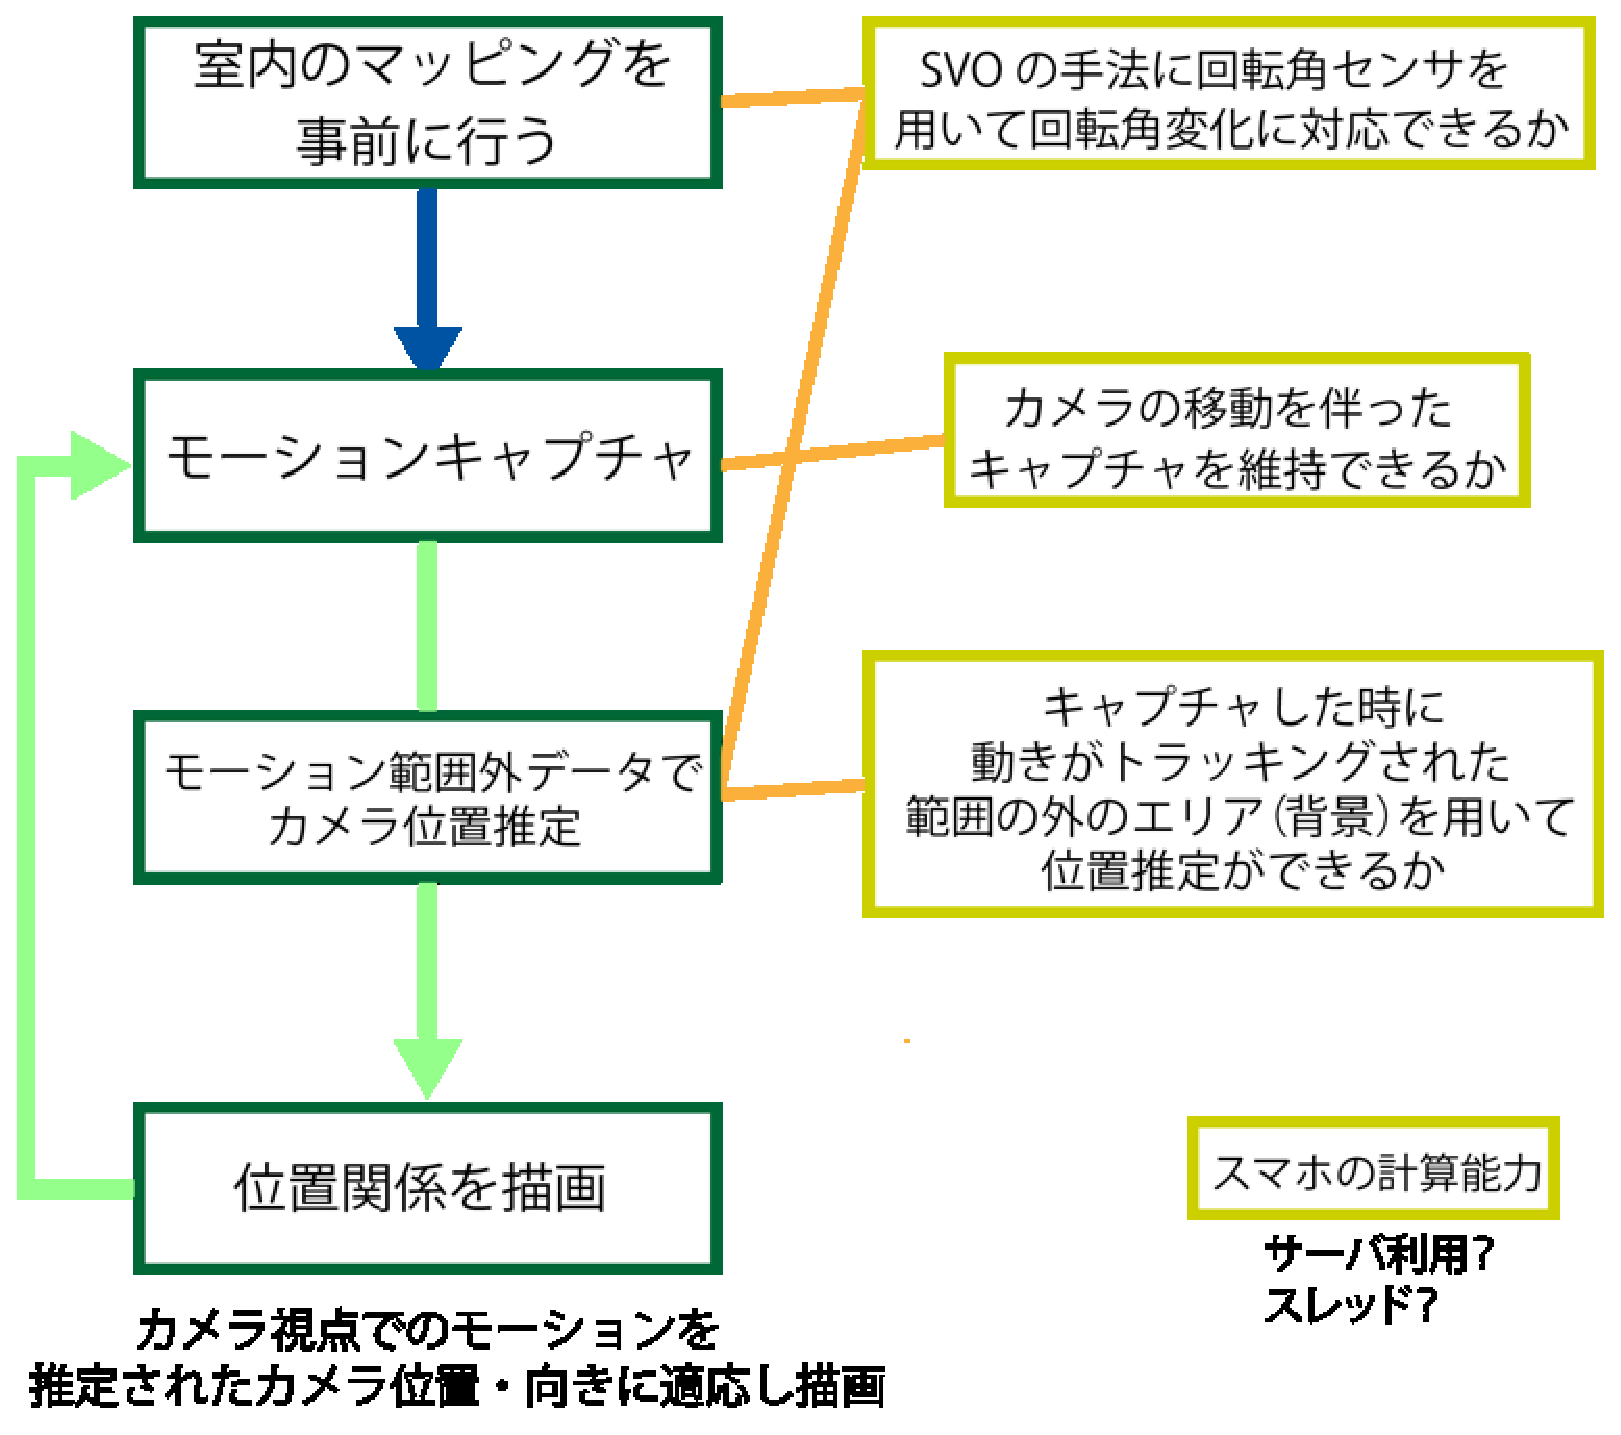
\includegraphics[scale = 0.5]{memo1.eps}
  \caption{提案手法の流れ(仮)}
  \label{method-fig}
\end{figure}

\chapter{参考文献}


%%%%%%%%%%%%%%%%%%%%%%%%%%%%%%%%%%%%%%%%%%%%%%%%%%%%%%%%%%%%%%%%%%%%%%%%

%%
%% 謝辞
%%
%% \begin{acknowledgements}
%% 感謝します.
%% \end{acknowledgements}

%%%%%%%%%%%%%%%%%%%%%%%%%%%%%%%%%%%%%%%%%%%%%%%%%%%%%%%%%%%%%%%%%%%%%%%%

%%
%% 参考文献
%%
\begin{thebibliography}{99}

\bibitem{wusethesis}
  福安直樹,
  卒業論文スタイルファイル(和歌山大学システム工学部用),\\
  \url{https://github.com/fukuyasu/wuse_thesis}.


\end{thebibliography}

%%%%%%%%%%%%%%%%%%%%%%%%%%%%%%%%%%%%%%%%%%%%%%%%%%%%%%%%%%%%%%%%%%%%%%%%

%%
%% 付録
%%
% \appendix
% 
% \chapter{サンプルプログラム}
% 
% プログラムリストや実行結果など,本論を補足する上で必要と思われるものが
% あれば付録として付ける.
% 
% {
% \footnotesize
% \begin{verbatim}
% #include <stdio.h>
% int main(void)
% {
%     printf("Hello, World!\n");
%     return 0;
% }
% \end{verbatim}
% }

%%%%%%%%%%%%%%%%%%%%%%%%%%%%%%%%%%%%%%%%%%%%%%%%%%%%%%%%%%%%%%%%%%%%%%%%

\end{document}
